\section{Pořizování 3D obrazu modelem dírkové kamery}
Při pořizování obrazu trojrozměrného (3D) světa kamerou se geometrie zobrazení reprezentuje modelem dírkové kamery (tj. 
perspektivní projekcí), ve kterém se 3D bod $(x,y,z)$ promítne do obrazové roviny jako $(x^{\prime},y^{\prime})$. 
Nakreslete odpovídající obrázek (stačí o dimenzi menší, tj. plošný). Předpokládejte, že znáte 3D souřadnice $(x,y,z)$, 
ohniskovou vzdálenost $f$, tj. vzdálenost obrazové roviny od středu promítání. Odvoďte vztah pro $x^{\prime}$.

\begin{figure}[H]
    \centering
    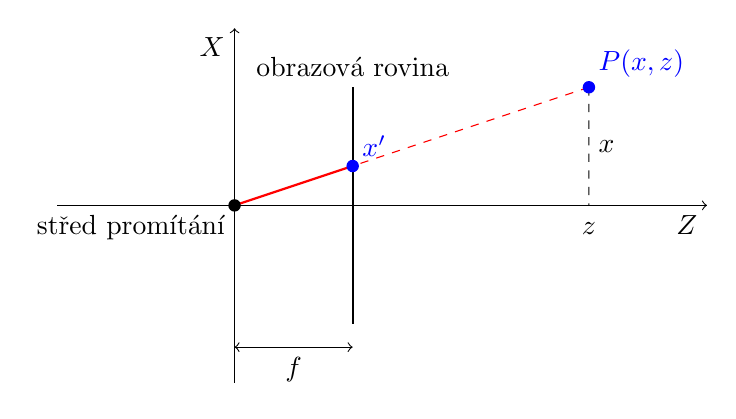
\begin{tikzpicture}[scale=1.5]
        % axis
        \draw[->] (-1.5,0) -- (4,0) node[below left] {$Z$};
        \draw[->] (0,-1.5) -- (0,1.5) node[below left] {$X$};

        % point in a scene and its projection
        \coordinate (P) at (3,1);
        \coordinate (O) at (0,0);
        \coordinate (P_prime) at (1,1/3);

        % image plane
        \draw[thick] (1,-1) -- (1,1) node[above] {obrazová rovina};

        % beam from point to projection center
        \draw[dashed, red] (P) -- (O);
        \draw[thick, red] (O) -- (P_prime);

        % distance labels
        \draw[<->] (1,-1.2) -- (0,-1.2) node[midway, below] {$f$};
        \draw[dashed] (P) -- (3,0) node[midway, right] {$x$};
        \draw[dashed] (P_prime) -- (1,0) node[midway, right] {};

        % point marks
        \fill[blue] (P) circle (1.5pt) node[above right] {$P(x,z)$};
        \fill[blue] (P_prime) circle (1.5pt) node[above right] {$x'$};
        \fill[black] (O) circle (1.5pt) node[below left] {střed promítání};

        \node at (3, -0.2) {$z$};
    \end{tikzpicture}
\end{figure}
Z podobnosti trojúhelníků plyne, že poměr jejich odpovídajících stran musí být stejný, tedy
\begin{align}
    \frac{x^\prime}{f} = \frac{x}{z} \\
    x^\prime = x \frac{f}{z}
\end{align}